\section{Стационарные и асинхронные ЭА.}

В обычных "поколенчатых" алгоритмах чтобы начать новую итерацию необходимо, чтобы приспособленность всей популяции поситалась. 

Бывает, что почти вся популяция обсчитана, кроме отдельных особей, для которых по каким-то причинам приспособленность считается долго. Тогда потоки/узлы, занимавшиеся другими особями проставиают => низкая эффективность использования распределенной системы.

\textbf{Решением данной проблемы являются асихронные ЭА}.

Сначала рассмотрим стационарные ЭА

\subsection*{Стационарные ЭА (по-английски - Steady-state)}
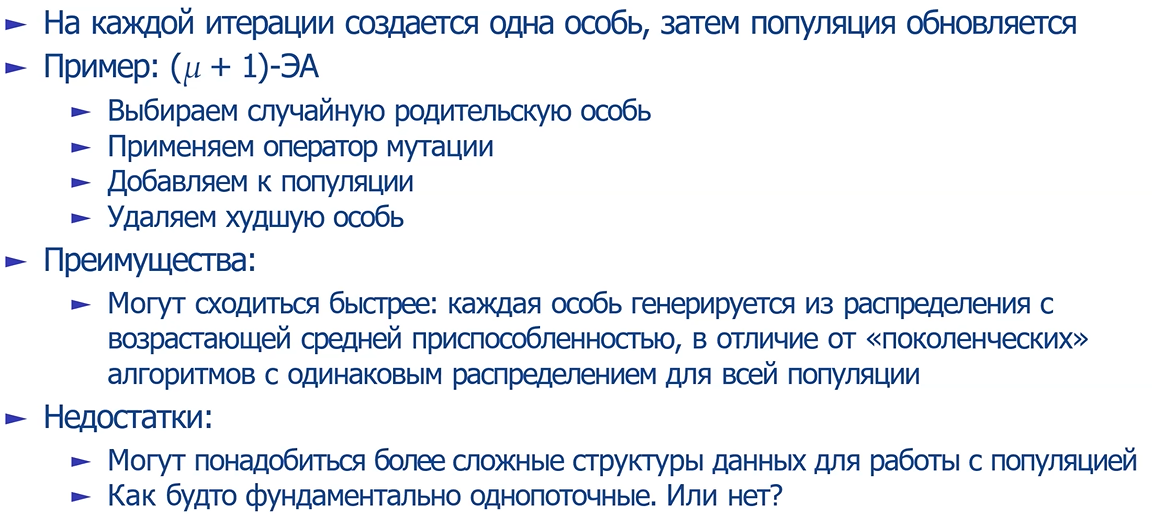
\includegraphics[width = 15cm]{images/68_steady_state.png}
\subsection*{Асинхронные ЭА}
Аналогичны steady-state, но не дожидаясь результатов функции приспособленности F1 новой особи L1 переходим к генерации следующей особи. Как только досчиталась F1 досчиталась, интегрируем L1 в текущую популяцию. В общем случае, пока считается F1 множество особей в популяции изменится, те L1 интегрируется не в ту же популяцию, из которой она генерировалась.

Такая адаптация позволяет применять распределенные вычисления и решает вышеописанную проблему.

\textbf{Особенности}
\begin{itemize}
    \item Генерация особей, обновление популяции - как в стационарных алгоритмах
    \item Асинхронные структуры данных => распараллеливание обновлений
    \item Асинхронность может сказаться на поведении алгоритма. В частности, может оказаться, что лучше выживают не более приспособленные особи, а те, которые быстрее обсчитываются (но эта проблема не обязательно возникает)
\end{itemize}

